\section{Preliminaries}

% \subsection{Conflict Graphs and Mazurkiewicz Traces}
% \begin{floatingfigure}{0.27\textwidth}
  \centering
  \tikzstyle{vertex}=[]
  \tikzstyle{arrow}=[thick, -latex]
  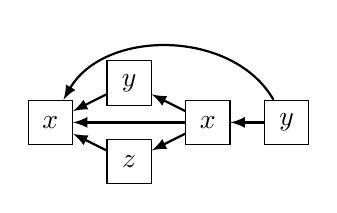
\begin{tikzpicture}
    \node[vertex] (x1) at (0, 0) {$x$};
    \node[vertex] (y1) at (1, 0.5) {$y$};
    \node[vertex] (y2) at (1, -0.5) {$z$};
    \node[vertex] (x2) at (2, 0) {$x$};
    \node[vertex] (z) at (3, 0) {$y$};

    \draw[arrow] (y1) to (x1);
    \draw[arrow] (y2) to (x1);
    \draw[arrow] (x2) to (y1);
    \draw[arrow] (x2) to (y2);
    \draw[arrow] (x2) to (x1);
    \draw[arrow, bend right=60] (z) to (x1);
    \draw[arrow] (z) to (x2);
  \end{tikzpicture}
  \caption{A conflict graph.}\figlabel{ExampleConflictGraph}
\end{floatingfigure}

%
% Consider a set $\Cmd$ of commands and a binary reflexive relation $\conflict$
% over $\Cmd$. We say two commands $x, y \in \Cmd$ \defword{conflict} if $(x, y)
% \in \conflict$, and we say they are \defword{independent} otherwise. A
% \defword{conflict graph}~\cite{mazurkiewicz1995introduction} (with respect to
% $\Cmd$ and $\conflict$) is a directed acyclic graph $C = (V, E, \varphi)$ where
% %
%   $V$ is a set of vertices;
% %
%   $E \subseteq V \times V$ is a set of edges;
% %
%   $\varphi: V \to \Cmd$ is a function that labels every vertex with a command;
%   and
% %
%   for every pair of vertices $v_1, v_2 \in V$, there exists an edge between
%   $v_1$ and $v_2$ if and only if $\varphi(v_1)$ and $\varphi(v_2)$ conflict.
% %
% We say $C' = (V', E', \varphi|_{V'})$ is a \defword{suffix} of $C$ if $C'$ is a
% subgraph of $C$ such that for every edge $(v_1, v_2) \in E$, if $v_1 \in V'$,
% then $(v_1, v_2) \in E'$.
% %
% An example conflict graph is shown in \figref{ExampleConflictGraph} with $\Cmd
% = \set{x, y, z}$ and $\conflict = \set{(x, x), (x, y), (y, x), (x, z), (z,
% x)}$. A suffix of this conflict graph is shown in \figref{ExampleSuffix}.
%
% We associate every conflict graph with the set of command strings that can be
% obtained by a reverse topological sort of the conflict graph. For example, the
% conflict graph in \figref{ExampleConflictGraph} can be reverse topological
% sorted in two ways, yielding the two command strings $xyzxy$ and $xzyxy$.
% Notice that these two command strings can be obtained from one another by
% interchanging their second and third commands, two commands that do not
% conflict. This is true in general. Any two command strings associated with a
% conflict graph can be obtained from the other by repeatedly interchanging
% adjacent independent commands. These sets of command strings are known as
% Mazurkiewicz traces~\cite{mazurkiewicz1985semantics,
% mazurkiewicz1995introduction} and formalize the orders in which replicated
% state machines can execute commands while remaining in sync.
%
% \subsection{Generalized Consensus}
% Generalized consensus~\cite{lamport1998part, sutra2011fast} involves a set of
% processes known as \defword{learners} attempting to reach consensus on a
% growing value. Though generalized consensus is defined in terms of an abstract
% data structure known as a command-structure set, we restrict our attention to
% generalized consensus on conflict graphs. More formally, given a set $\Cmd$ of
% commands and conflict relation $\conflict$, we consider a set $l_1, l_2,
% \ldots, l_n$ of learners where each learner $l_i$ manages a conflict graph
% $C_i$. Over time, a set of client processes propose commands, and learners add
% the proposed commands to their conflict graphs such that the following four
% conditions are maintained.
% \begin{itemize}
%   \item \defword{Nontriviality:}
%     The vertices of every conflict graph are labelled only with proposed
%     commands.
%   \item \defword{Stability:}
%     Every conflict graph $C_i$ at time $t$ is a suffix of $C_i$ at any time after
%     $t$.
%   \item \defword{Consistency:}
%     For every pair of conflict graphs $C_i$ and $C_j$, there exists a conflict
%     graph $C$ such that $C_i$ and $C_j$ are both suffixes of $C$.
%   \item \defword{Liveness:}
%     If a command is proposed, then eventually every conflict graph contains it.
% \end{itemize}

\subsection{BPaxos Graphs and Partial BPaxos Graphs}
\begin{figure}[ht]
  \centering
  \tikzstyle{vertex}=[draw, minimum width=16pt, minimum height=16pt]
  \tikzstyle{arrow}=[thick, -latex]

  \begin{subfigure}[b]{2in}
    \centering
    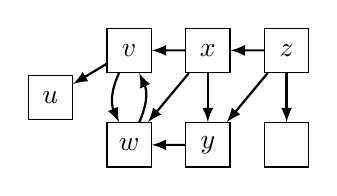
\begin{tikzpicture}[xscale=1, yscale=0.6]
      \node[vertex] (u) at (0, 0) {$u$};
      \node[vertex] (v) at (1, 1) {$v$};
      \node[vertex] (w) at (1, -1) {$w$};
      \node[vertex] (x) at (2, 1) {$x$};
      \node[vertex] (y) at (2, -1) {$y$};
      \node[vertex] (z) at (3, 1) {$z$};
      \node[vertex] (unknown) at (3, -1) {\phantom{z}};

      \draw[arrow] (v) to (u);
      \draw[arrow, bend right=15] (v) to (w);
      \draw[arrow, bend right=15] (w) to (v);
      \draw[arrow] (x) to (v);
      \draw[arrow] (x) to (w);
      \draw[arrow] (x) to (y);
      \draw[arrow] (y) to (w);
      \draw[arrow] (z) to (x);
      \draw[arrow] (z) to (y);
      \draw[arrow] (z) to (unknown);
    \end{tikzpicture}
    \caption{A partial BPaxos graph $B$}\figlabel{PartialBPaxosGraph}
  \end{subfigure}%
  \begin{subfigure}[b]{2in}
    \centering
    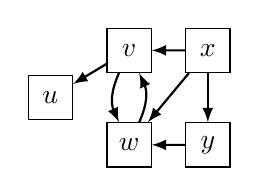
\begin{tikzpicture}[xscale=1, yscale=0.6]
      \node[vertex] (u) at (0, 0) {$u$};
      \node[vertex] (v) at (1, 1) {$v$};
      \node[vertex] (w) at (1, -1) {$w$};
      \node[vertex] (x) at (2, 1) {$x$};
      \node[vertex] (y) at (2, -1) {$y$};

      \draw[arrow] (v) to (u);
      \draw[arrow, bend right=15] (v) to (w);
      \draw[arrow, bend right=15] (w) to (v);
      \draw[arrow] (x) to (v);
      \draw[arrow] (x) to (w);
      \draw[arrow] (x) to (y);
      \draw[arrow] (y) to (w);
    \end{tikzpicture}
    \caption{The eligibile suffix $B'$ of $B$}\figlabel{EligibleSuffix}
  \end{subfigure}%
  \begin{subfigure}[b]{2in}
    \centering
    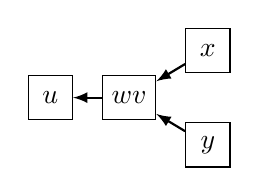
\begin{tikzpicture}[xscale=1, yscale=0.6]
      \node[vertex] (u) at (0, 0) {$u$};
      \node[vertex] (vw) at (1, 0) {$wv$};
      \node[vertex] (x) at (2, 1) {$x$};
      \node[vertex] (y) at (2, -1) {$y$};

      \draw[arrow] (vw) to (u);
      \draw[arrow] (x) to (vw);
      \draw[arrow] (y) to (vw);
    \end{tikzpicture}
    \caption{The condensation of $B'$}\figlabel{Condensation}
  \end{subfigure}

  \caption{}
\end{figure}


Consider again a set $\Cmd$ of commands and a conflict relation $\conflict$. A
\defword{BPaxos graph} (with respect to $\Cmd$ and $\conflict$) is a directed
(potentially cyclic) graph $B = (V, E, \varphi)$ where
%
  $V$ is a set of vertices;
%
  $E \subseteq V \times V$ is a set of edges;
%
  $\varphi: V \to \Cmd$ is a function that labels every vertex with a command;
  and
%
  for every pair of vertices $v_1, v_2 \in V$, there exists an edge between
  $v_1$ and $v_2$ if (but not only if) $\varphi(v_1)$ and $\varphi(v_2)$
  conflict.
%
Intuitively, a BPaxos graph is a potentially cyclic conflict graph that can
have spurious edges between vertices labelled with non-conflicting commands.

A \defword{partial BPaxos graph} $B = (V, E, \varphi)$ is a BPaxos graph except
that $\varphi: V \partialto \Cmd$ is partial. Intuitively, a partial BPaxos
graph is a BPaxos graph for which the labels of some vertices are unknown.
%
We say a vertex $v$ in a partial BPaxos graph is \defword{eligible} if $v$ and
all vertices reachable from $v$ are labelled. The \defword{eligible suffix} of
a partial BPaxos graph $B$ is the suffix of $B$ consisting of all eligible
vertices.
%
An example partial BPaxos graph is illustrated in \figref{PartialBPaxosGraph},
and its eligible suffix is shown in \figref{EligibleSuffix}.

The \defword{condensation} of BPaxos graph $B$ is the graph obtained by first
removing spurious edges between non-conflicting vertices in $B$ and then by
contracting every strongly connected component. Every strongly connected
component labelled with commands $x_1, \ldots, x_n$ is replaced with a single
vertex labelled with a command string $x_{i_1} x_{i_2} \cdots x_{i_n}$ that is
obtained from an arbitrary but fixed ordering of the commands $x_1, \ldots,
x_n$. An example condensation is shown in \figref{Condensation}.
%
The condensation of a BPaxos graph with respect to $\Cmd$ and $\conflict$ is
a conflict graph with respect to $\Cmd^+$ and $\conflict^+$ where $\Cmd^+$ is
the set of non-empty command strings and where $(x_1 x_2 \cdots x_n, y_1 y_2
\cdots y_m) \in \conflict^+$ if there is some $x_i$ and $y_j$ that conflict in
$\conflict$.

\subsection{Paxos and Fast Paxos}
\begin{figure}[ht]
  \begin{minipage}[t]{0.48\textwidth}
    \begin{algorithm}[H]
      \caption{Fast Paxos Phase 2a}%
      \algolabel{FastPaxos}
      \begin{algorithmic}[1]
        \State $M \gets$ phase 1b messages from a quorum $\Quorum$
        \State $k \gets$ the largest vote round in $M$
        \State $V \gets$ the vote values in $M$ for round $k$
        \If{$k = -1$}\linelabel{FastPaxosCase1}
          \State send any proposed value \linelabel{FastPaxosCase1Code}
        \ElsIf{$V = \set{v}$}\linelabel{FastPaxosCase2}
          \State send $v$ \linelabel{FastPaxosCase2Code}
        \ElsIf{$\exists v \in V.\ O4(v)$}\linelabel{FastPaxosCase3}
          \State send $v$ \linelabel{FastPaxosCase3Code}
        \Else{}\linelabel{FastPaxosCase4}
          \State send any proposed value \linelabel{FastPaxosCase4Code}
        \EndIf{}
      \end{algorithmic}
    \end{algorithm}
  \end{minipage}%
  \hspace{0.04\textwidth}%
  \begin{minipage}[t]{0.48\textwidth}
    \begin{algorithm}[H]
      \caption{Fast Paxos Phase 2a Tweak}%
      \algolabel{FastPaxosTweak}
      \begin{algorithmic}[1]
        \State $M \gets$ phase 1b messages from a quorum $\Quorum$
        \State $k \gets$ the largest vote round in $M$
        \State $V \gets$ the vote values in $M$ for round $k$
        \If{$k = -1$}\linelabel{FastPaxosTweakCase1}
          \State send 2a with any proposed value \linelabel{FastPaxosTweakCase1Code}
        \ElsIf{$k \neq 0$}\linelabel{FastPaxosTweakCase2}
          \State send 2a with unique $v \in V$ \linelabel{FastPaxosTweakCase2Code}
        \ElsIf{$\exists v \in V$ maybe chosen in round $0$}\linelabel{FastPaxosTweakCase3}
          \State send 2a with $v$ \linelabel{FastPaxosTweakCase3Code}
        \Else{}\linelabel{FastPaxosTweakCase4}
          \State send 2a with any proposed value \linelabel{FastPaxosTweakCase4Code}
        \EndIf{}
      \end{algorithmic}
    \end{algorithm}
  \end{minipage}
\end{figure}

Fast Paxos~\cite{lamport2006fast} is a two-phase consensus algorithm structured
around a set of clients, leaders, acceptors, and learners. For a full
description of Fast Paxos, we defer the reader to \cite{lamport2006fast}, but
we highlight the salient bits of Fast Paxos here. Fast Paxos proceeds in a
series of integer-valued rounds with $0$ being the smallest round and $-1$
being a null round. In phase 2a of the algorithm, a leader has to choose a
value to send to the acceptors. The logic for choosing this value is shown in
\algoref{FastPaxos} where $O4(v)$ is true if there exists a fast quorum
$\FastQuorum$ of acceptors such that every acceptor in $\FastQuorum \cap
\Quorum$ voted for $v$ in round $k$.
%
If we assume that round $0$ is a fast round and every other round is a classic
round, we can modify phase 2a as shown in \algoref{FastPaxosTweak}. The process
of determining whether a value $v$ in \lineref{FastPaxosTweakCase3} of
\algoref{FastPaxosTweak} may have been chosen in round $0$ is left
intentionally abstract. We will see later that different BPaxos Protocols will
implement \lineref{FastPaxosTweakCase3} in different ways. The correctness proof
of this alternative phase 2a is a straightforward modification of the proof
given in \cite{lamport2006fast}.
